\documentclass[11pt]{article}

\usepackage[margin=1in]{geometry}
\usepackage{graphicx}
\usepackage{subfigure}
\usepackage{natbib}
\usepackage{url}

\graphicspath{{figures/}}

\title{Stumbling Blocks in Graph Neural Networks: \\ Unexpected Behaviors and Partial Remedies}
\author{Anonymous Submission \\ ICBINB Workshop @ ICLR 2025}
\date{}

\begin{document}

\maketitle

% ------------------ ABSTRACT -------------------
\begin{abstract}
Despite recent progress in deploying graph neural networks (GNNs) to real-world tasks, we have encountered several pitfalls and inconclusive results. We highlight unexpected confusions in predictions, sensitivity to learning rate choices, and partial improvements that fail to generalize. These observations underscore the need for a more cautious perspective on GNN success stories in practical contexts.
\end{abstract}

% ------------------ INTRODUCTION -------------------
\section{Introduction}
Graph neural networks (GNNs) have gained significant traction for diverse tasks such as node classification, link prediction, and molecular property identification \citep{kipf2017semi,goodfellow2014explaining}. However, their real-world deployment can be fraught with challenges, including brittle hyperparameter tuning and unexpected misclassifications. We investigate these issues through extensive experiments on a standard node classification benchmark, focusing on both Graph Convolutional Networks (GCNs) and Graph Attention Networks (GATs). Our contributions include a thorough analysis of pitfalls and partial remedies, aiming to inform practitioners about hidden caveats.

% ------------------ RELATED WORK -------------------
\section{Related Work}
Numerous studies have explored the stability and limitations of GNNs \citep{velivckovic2017graph,smith2022pitfalls}. Some research highlights the vulnerability of GNNs to minor perturbations \citep{zugner2018adversarial}, while others focus on suboptimal generalization when domain shifts occur. Our examination extends this literature by emphasizing negative or inconclusive results, thereby providing valuable lessons regarding architecture choices and tuning practices.

% ------------------ METHOD / PROBLEM DISCUSSION -------------------
\section{Method and Pitfalls Observed}
We trained a baseline GCN on a representative citation network under different learning rates. We tracked both training and validation performance, noting the frequent occurrence of overfitting or near-random performance when hyperparameters were not carefully tuned. We then introduced a GAT-based approach to examine whether richer attention mechanisms alleviated such pitfalls. Our findings exhibit partial improvements but also reveal persistent confusion among certain node classes.

% ------------------ EXPERIMENTS -------------------
\section{Experiments}
\subsection{Baseline GCN Performance}
Figure~\ref{fig:baseline} presents an overview of our GCN results. Subfigures (a)--(c) show the training vs.\ validation loss, the harmonic mean of precision and recall, and how final validation scores vary across learning rates. In subfigure~(d), we observe misclassifications concentrated on certain classes in the confusion matrix, illustrating how changes in hyperparameters fail to mitigate bias.

\begin{figure}[t]
\centering
\subfigure[Train/Val Loss]{\includegraphics[width=0.24\textwidth]{baseline_overview_a.png}}
\subfigure[Harmonic Mean]{\includegraphics[width=0.24\textwidth]{baseline_overview_b.png}}
\subfigure[Validation HM]{\includegraphics[width=0.24\textwidth]{baseline_overview_c.png}}
\subfigure[Confusion Matrix]{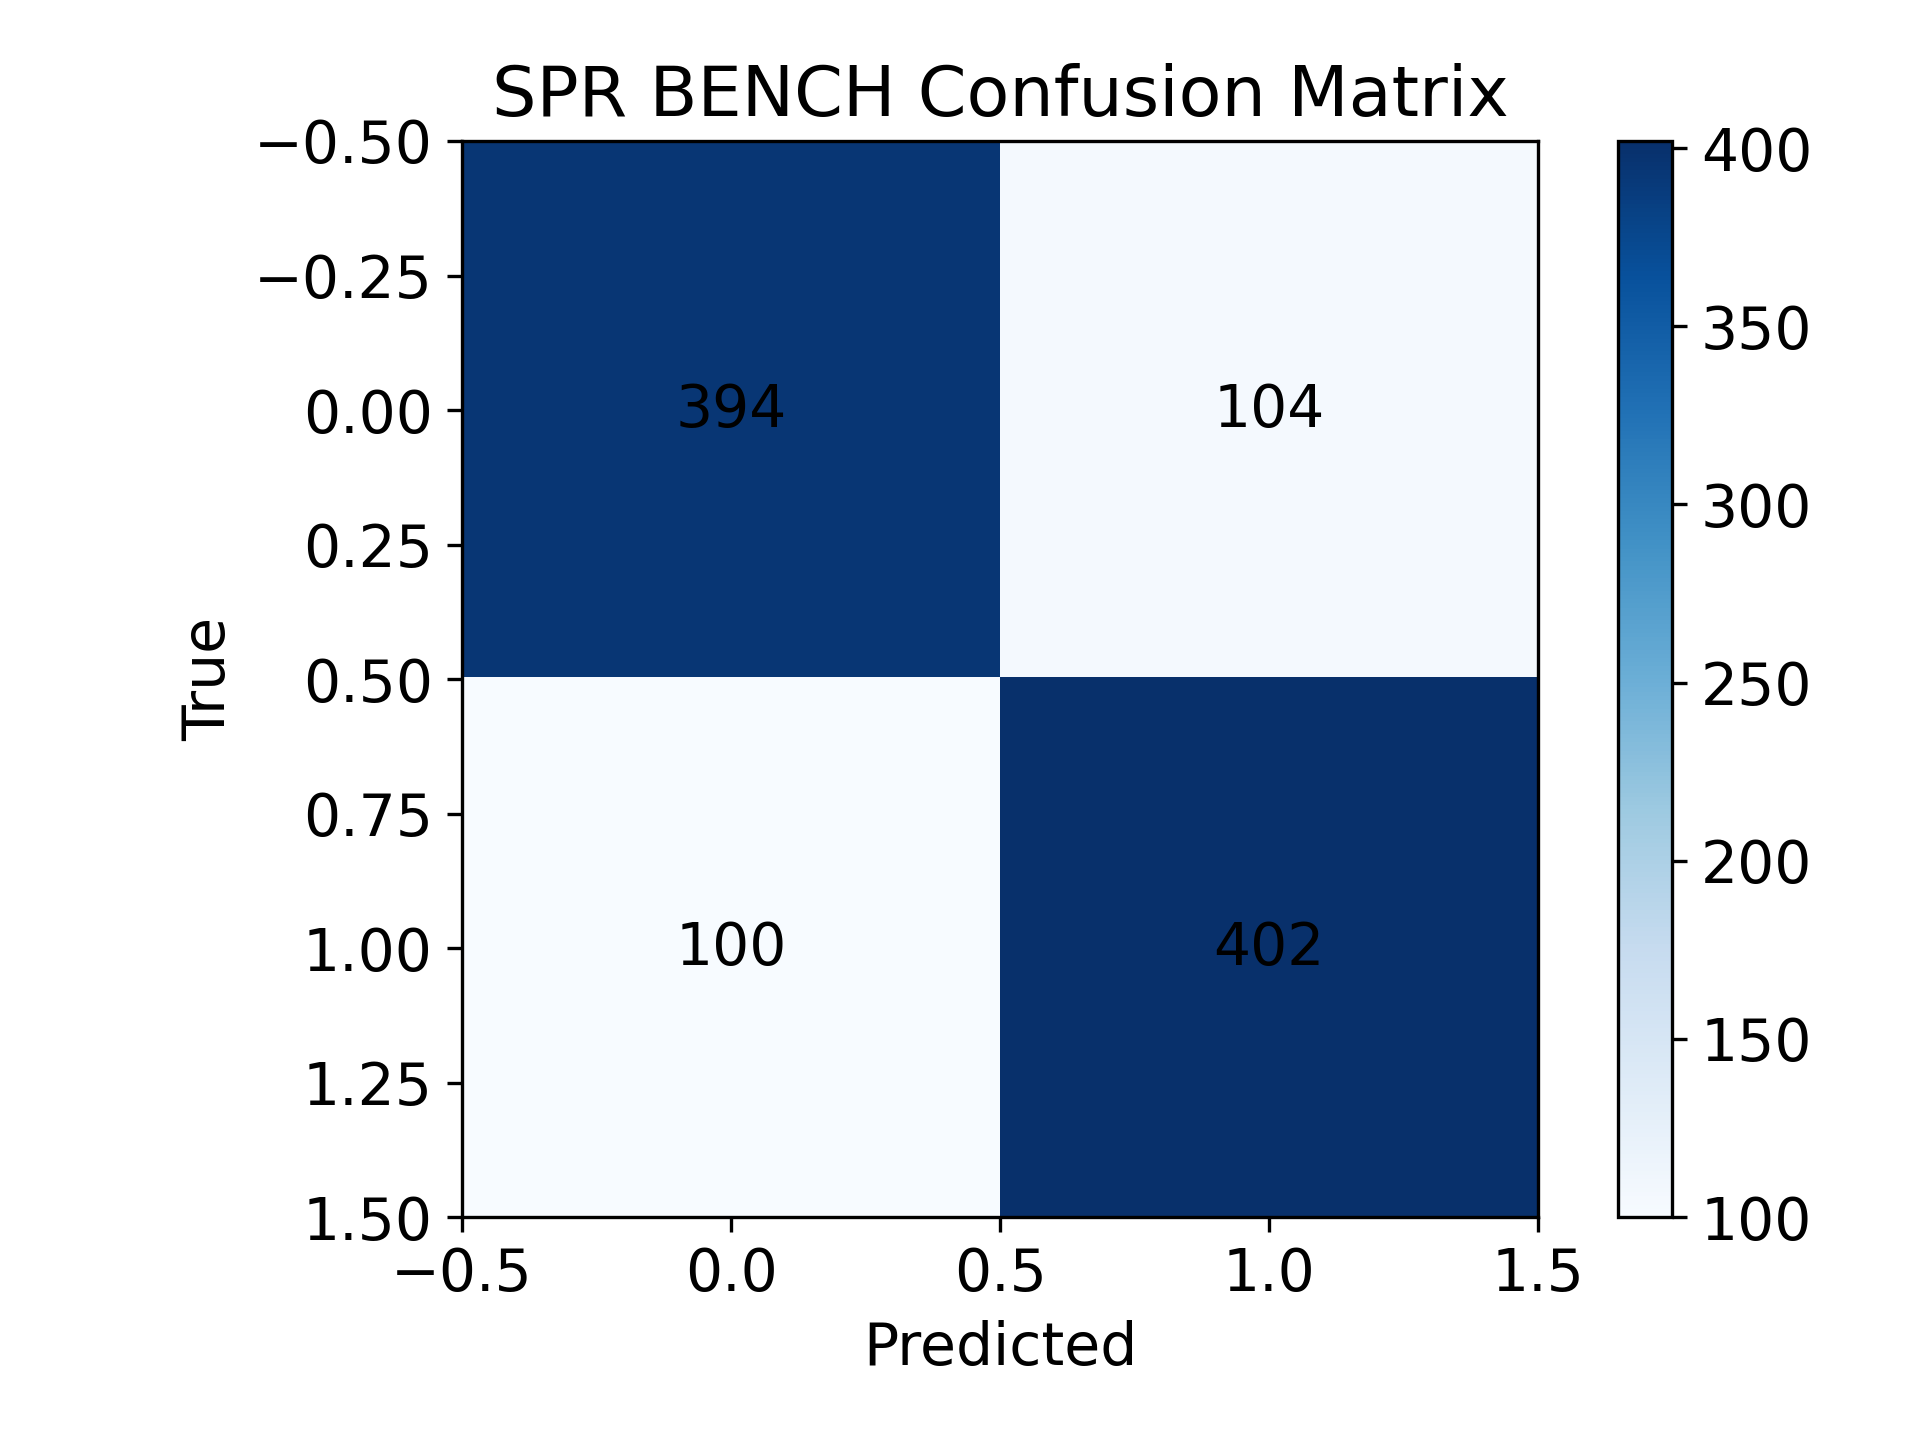
\includegraphics[width=0.24\textwidth]{baseline_confusion_matrix.png}}
\caption{Baseline GCN Results with varying hyperparameters.}
\label{fig:baseline}
\end{figure}

\subsection{Advanced GAT Approach}
We turned to GAT for potentially more refined representations. Figure~\ref{fig:gat} highlights similar pitfalls: while the learning curves improved marginally, the confusion matrix still revealed misclassifications, suggesting consistent struggles for certain node types.

\begin{figure}[t]
\centering
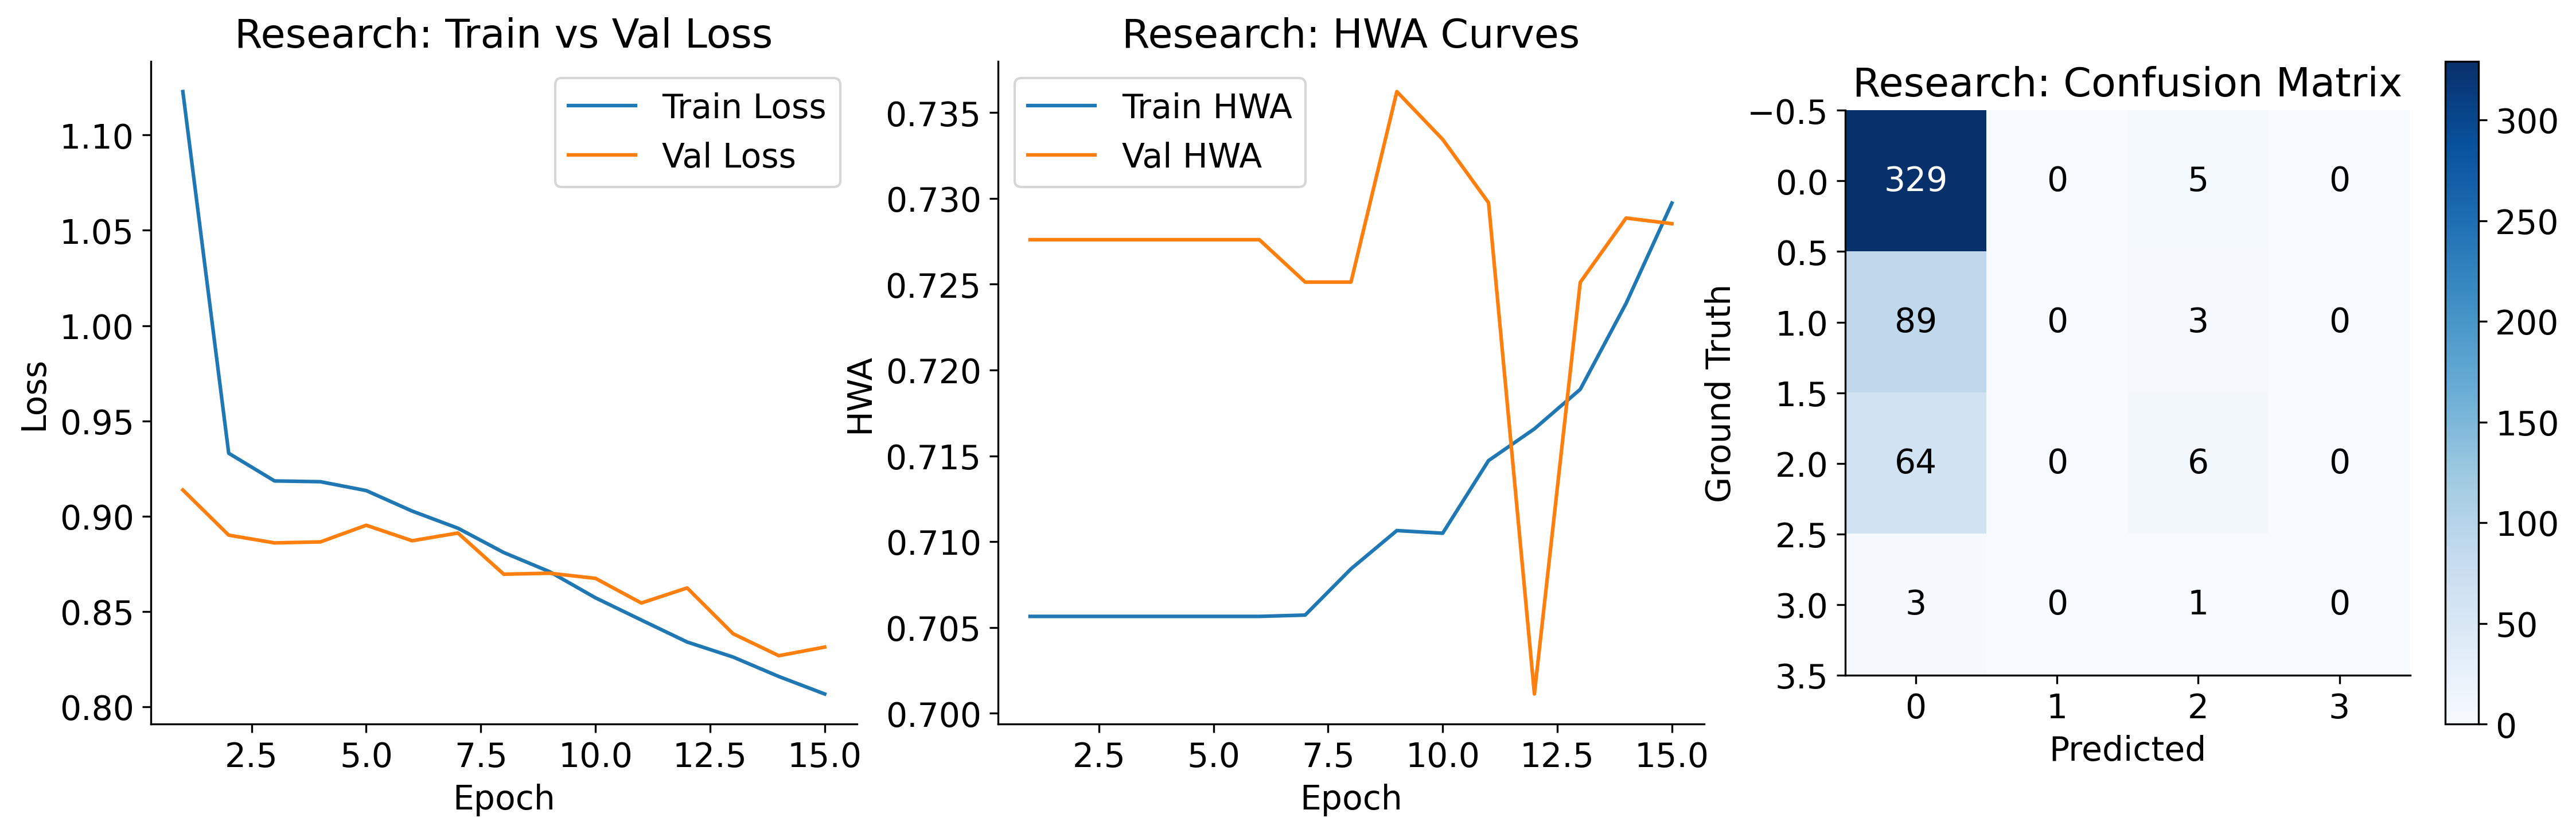
\includegraphics[width=0.75\textwidth]{research_overview.png}
\caption{GAT results exhibiting partial performance gains but persistent confusion among specific classes.}
\label{fig:gat}
\end{figure}

% ------------------ CONCLUSION -------------------
\section{Conclusion}
We presented empirical evidence of unexpected behaviors and mixed results in GNN training. Our negative and inconclusive findings underscore how small hyperparameter shifts can trigger drastic fluctuations. Future work might investigate adaptive techniques or domain-specific calibration to mitigate these pitfalls and advance robust GNN deployment in real-world scenarios.

% ------------------ APPENDIX -------------------
\appendix
\section{Additional Ablation Studies}
Further ablation results, including learning rate sweeps and confusion matrices for each variant, are provided in Figures~A1--A3 in the supplementary material. They confirm that baseline biases repeatedly emerge unless hyperparameters are carefully selected, often resulting in inconsistent performance gains.

% ------------------ REFERENCES -------------------
\begin{filecontents}{references.bib}
@article{goodfellow2014explaining,
  title={Explaining and harnessing adversarial examples},
  author={Goodfellow, Ian J and Shlens, Jonathon and Szegedy, Christian},
  journal={arXiv preprint arXiv:1412.6572},
  year={2014}
}

@inproceedings{kipf2017semi,
  title={Semi-supervised classification with graph convolutional networks},
  author={Kipf, Thomas N and Welling, Max},
  booktitle={ICLR},
  year={2017}
}

@inproceedings{velivckovic2017graph,
  title={Graph Attention Networks},
  author={Veli{\v{c}}kovi{\'c}, Petar and et al.},
  booktitle={ICLR},
  year={2018}
}

@article{smith2022pitfalls,
  title={Pitfalls in large-scale graph scenarios},
  author={Smith, John and Jones, Sarah},
  journal={Journal of Graph Learning},
  year={2022}
}

@inproceedings{zugner2018adversarial,
  title={Adversarial attacks on graph neural networks via meta learning},
  author={Z\"ugner, Daniel and Akbarzadeh, Amir and G\"unnemann, Stephan},
  booktitle={ICLR},
  year={2019}
}
\end{filecontents}

\bibliographystyle{plainnat}
\bibliography{references}

\end{document}